\documentclass[11pt,a4paper]{article}
\usepackage[margin=1in]{geometry}
\usepackage[T1]{fontenc}
\usepackage{lmodern}
\usepackage{microtype}
\usepackage{booktabs}
\usepackage{longtable,array,amsmath,amssymb}
\usepackage{caption}
\captionsetup{font=small,labelfont=bf}
\usepackage{tikz,pgfplots}
\pgfplotsset{compat=1.18}
\usepackage{xurl,hyperref}
\hypersetup{hidelinks}
\setlength{\parindent}{0pt}
\setlength{\parskip}{5pt}
\setlength{\tabcolsep}{3pt}
\renewcommand{\arraystretch}{1.1}
\newcolumntype{L}[1]{>{\raggedright\arraybackslash}p{#1}}
\newcolumntype{R}[1]{>{\raggedleft\arraybackslash}p{#1}}
\begin{document}
% FORMAT [P2]: MCM context retained; generated hierarchy, captions and cross-references.
% Protected: numerical outputs and input data. Meaning-Check: PRESERVED. Risk-Flags: none.
\begin{center}
{\Large\bfseries A Budget-Constrained Forecast of Olympic Medal Tables\par}
\medskip Summary Sheet | 2025 MCM Problem C | Training reconstruction
\end{center}
2025 MCM Problem C | Training reconstruction | Analysis date: 9 October 2026

We use only the five supplied datasets to construct delegation-edition targets, compare six forecasting strategies, and generate joint 2028 gold and total-medal distributions. National targets come from the official medal table; athlete records supply historical participation and sport proxies.

On rolling forecasts for 2008, 2012, 2016 and 2020, the weighted-history benchmark has the lowest point-error score: total MAE 1.475 and gold MAE 0.679. The anchored first-medal hurdle has MAE 1.661 and 0.740. We retain the benchmark and use the hurdle for the additional host, first-medal and joint-distribution tasks, without claiming it is the best point predictor.

Our primary 2028 scenario retains the 2024 roster, programme and reported-delegation medal budgets: 205 delegations, 328 gold and 1039 total medals. Every simulated outcome satisfies these budgets and gold no greater than total. The USA has expected gold 46.6, total 141.2; China has gold 37.2, total 86.8. Intervals are broad, reflecting historical dispersion and edition-cluster parameter uncertainty.

Among 65 historically unmedalled candidate delegations, the expected first-medal count is 3.38, with a 95\% predictive range 0-7. The most likely count is 3, probability 21.7\%. Sport reallocation and coaching investments are explicit scenarios, not known 2028 programme changes or identified coaching causal effects.

The supplied programme stops at 2024 and includes no coach appointment records. We disclose measurement disagreement, roster uncertainty, retrospective model development, and scenario assumptions. This AI-assisted reconstruction is supported by saved code, outputs and verification records \cite{comap-problem,comap-data,nb2-doc}.

\clearpage
\tableofcontents
\clearpage
\section{Data and scope}
The official ZIP and local CSV files are byte-identical. The raw athlete file has 252,565 rows; 1,466 exact duplicate rows are removed. We map 164 medal-table names to the supplied delegation codes and construct 3,226 delegation-edition records.

Medal-table NOC values are country names, whereas athlete NOC values are codes. We use normalized supplied Team labels and documented aliases. FR Yugoslavia in 1996/2000 aligns to SCG; Lebanon LBN and LIB are reconciled using the same Team label. Predecessor states are not redistributed to successor countries. Mixed, refugee and neutral delegations are not presented as sovereign countries.

Country gold and total targets use the official table. A missing aggregate is zero only when no athlete medal is recorded; inconsistent medal-bearing rows remain unresolved and are excluded from supervised labels. AIN 2024 and MDA 2012 are the modern unresolved cases. The current scenario excludes AIN because its official aggregate is absent.

Deduplicated team-event medal-unit proxies exactly reproduce the official total for 599/673 comparable modern delegation-editions. We therefore label sport measures as proxies. Compound sport labels are grouped where possible; genuinely mixed categories remain explicit.

Athlete names are not unique identifiers. Name-based participant counts are approximate. Future participation, athletes and event counts are not observed. The supplied host file identifies the USA in 2028; the programme has no 2028 column \cite{comap-problem,comap-data}.

Table~\ref{tab:1} records the input contract.

\begin{table}[htbp]
\centering
\caption{Supplied inputs and their modelling roles.}
\label{tab:1}
\small
\begin{tabular}{@{}L{4.122cm} R{6.107cm} R{5.038cm}@{}}
\toprule
Input & Rows & Role\\
\midrule
Athletes & 252565 & Participation and sport proxy\\
Medal counts & 1435 & Official national targets\\
Hosts & 35 & Known host indicator\\
Programme & 74 & Historical event opportunities\\
Dictionary & Not a modelling table & Definitions and special symbols\\
\bottomrule
\end{tabular}
\end{table}
\section{Forecasting model}
All historical predictors use editions earlier than the target. The forecast roster is the preceding edition roster with valid targets; target nonparticipants are scored as zero outcomes, not assumed zero ability. New entrants outside this roster are not predicted. We train from 1996 and evaluate 2008 onward.

The method proceeds from verified national targets to lagged features, established/first-medal count draws, conditional gold draws, and joint budget allocation. Rolling comparisons evaluate the predictive modules; budget tests evaluate outcome coherence. The equations below follow this same input-to-output order.

Weighted history is 0.6 times the preceding medal total, 0.3 times two editions ago and 0.1 times three editions ago. General Poisson and NB2 regressions use log historical medals, log historical participant count, historical sport breadth, current and preceding host flags, and a clipped historical trend. NB2 variance is mu + alpha*mu\textasciicircum{}2 \cite{nb2-doc}.

For previously medalled delegations, the anchored hurdle uses weighted history as an offset, adding a small support term 0.05 and learned current/prior-host corrections. The fitted log coefficients are 0.0971, 0.1594, -0.0743; NB dispersion alpha=0.1536. Regularization and bounds are recorded in source.

For previously unmedalled delegates, logistic regression predicts first-medal probability from prior participant count, participant trend and observed past Games. Conditional positive counts use a zero-truncated NB draw. Gold is sampled conditional on total using the recent gold share (pooled one-third if no historical total); gold cannot exceed total.

We refit 80 edition-cluster bootstrap samples and generate 20,000 future draws. Hamilton largest-remainder allocation separately redistributes gold and non-gold to fixed supplied 2024 budgets. It preserves integer totals and zero support and induces cross-country competition. Quantile intervals summarize the allocated joint draws.

These future intervals combine parameter resampling and outcome dispersion conditional on the roster and budget scenario. They do not cover unknown policy changes, data errors or all possible 2028 schedules. The historical process-only and joint-budget checks are reported separately.

\begin{equation}
W_{i,t}=0.6T_{i,t-4}+0.3T_{i,t-8}+0.1T_{i,t-12}\label{eq:1}
\end{equation}
Weighted official totals define the historical reference W. Edition labels are four years apart; 2020 denotes the postponed Games held in 2021.
\begin{equation}
\mu_{i,t}=(W_{i,t}+0.05)\exp(\beta_0+\beta_H H_{i,t}+\beta_P H_{i,t-4})\label{eq:2}
\end{equation}
For previously medalled delegations, H is the supplied current or preceding host indicator. This mean feeds the negative-binomial outcome draw.
\begin{equation}
q_{i,t}=\mathrm{logistic}(\boldsymbol{\gamma}^{\mathsf{T}}\mathbf{x}_{i,t})\label{eq:3}
\end{equation}
For historically unmedalled delegations, x contains an intercept, log participant scale, clipped participant trend and log observed Games. q is the pre-allocation first-medal probability.
\begin{equation}
Y_{i,t}\sim\mathrm{NB2}(\mu_{i,t},\alpha),\quad\mathrm{Var}(Y)=\mu+\alpha\mu^2\label{eq:4}
\end{equation}
NB2 describes overdispersed counts. For rare delegations, the general historical-feature NB mean and dispersion feed a zero-truncated draw instead of the anchored established-delegation mean.
\begin{equation}
\mathrm{E}[Y_{i,t}\mid\mathrm{rare}]=q_{i,t}\frac{\mu_{i,t}}{1-(1+\alpha\mu_{i,t})^{-1/\alpha}}\label{eq:5}
\end{equation}
The hurdle sets Y to zero when no breakthrough is drawn, and otherwise draws a positive NB count. The expectation is before global allocation.
\begin{equation}
X_{i,t}\mid Y_{i,t}\sim\mathrm{Binomial}(Y_{i,t},s_{i,t})\label{eq:6}
\end{equation}
The recent weighted gold share s, clipped to [0.001,0.999] with pooled fallback 1/3, produces raw gold X. Gold and non-gold weights then enter separate integer allocations.
\begin{equation}
\sum_i G_{i,t}=328,\quad\sum_i T_{i,t}=1039,\quad0\leq G_{i,t}\leq T_{i,t}\label{eq:7}
\end{equation}
Final G and T are allocated gold and total medals. These budgets are the supplied 2024 reported-delegation aggregates, excluding the unreported AIN aggregate.
\section{Rolling validation}
We compare all six models under the same previous-roster forecasting protocol. Mean metrics below are calculated on 2008, 2012, 2016 and 2020. MAE is per delegation; pooled averages are heavily influenced by small delegations, so RMSE and individual outputs are also saved.

Weighted history remains the strongest point benchmark. A hurdle is needed for nonzero first-medal probabilities and the selected anchored variant has lower joint error than the general NB hurdle. Selection combines total MAE, gold MAE and first-medal Brier among task-complete hurdle models. This restricted selection is not evidence that the chosen model wins unrestricted point prediction.

For 2024, the anchored model has total MAE 1.555, gold MAE 0.700, total RMSE 4.210 and gold RMSE 1.780. Process-only 95\% coverage is 96.1\% for total and 96.1\% for gold. These broad intervals are conservative, not a claim of sharp precision.

2024 benchmark results were inspected during development before adding the anchored model. We disclose it as a retrospective check rather than an untouched confirmatory holdout. Gold/total budget allocation is also checked retrospectively while retaining the preceding edition budget, not the actual target medal total.

Figure~\ref{fig:1} provides the corresponding visual comparison.

Table~\ref{tab:2} reports the numerical results.

\begin{table}[htbp]
\centering
\caption{Rolling validation errors and first-medal Brier scores; lower values are better.}
\label{tab:2}
\small
\begin{tabular}{@{}L{5.119cm} R{3.312cm} R{3.312cm} R{3.312cm}@{}}
\toprule
Model & Total MAE & Gold MAE & First Brier\\
\midrule
weighted & 1.475 & 0.679 & 0.057\\
last & 1.497 & 0.696 & 0.057\\
poisson & 1.643 & 0.714 & 0.083\\
anchored\_hurdle & 1.661 & 0.740 & 0.053\\
nb\_first\_hurdle & 1.820 & 0.728 & 0.053\\
negative\_binomial & 1.864 & 0.744 & 0.066\\
\bottomrule
\end{tabular}
\end{table}
\begin{figure}[htbp]
\centering
\begin{center}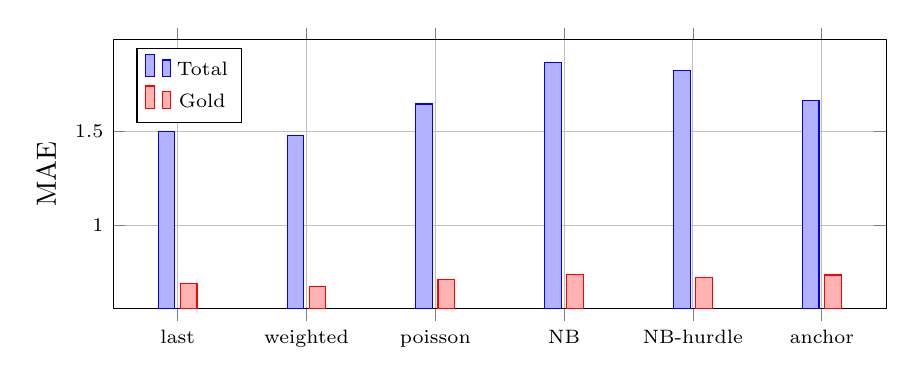
\begin{tikzpicture}\begin{axis}[width=0.94\linewidth,height=5cm,grid=major,legend style={font=\scriptsize},tick label style={font=\scriptsize},ybar,bar width=6pt,symbolic x coords={last,weighted,poisson,NB,NB-hurdle,anchor},xtick=data,ylabel={MAE},legend pos=north west]
\addplot coordinates {(last,1.4970) (weighted,1.4749) (poisson,1.6429) (NB,1.8639) (NB-hurdle,1.8196) (anchor,1.6608)};
\addplot coordinates {(last,0.6965) (weighted,0.6787) (poisson,0.7136) (NB,0.7437) (NB-hurdle,0.7278) (anchor,0.7397)};
\legend{Total,Gold}
\end{axis}\end{tikzpicture}\end{center}

\caption{Rolling validation compares per-delegation errors across the 2008--2020 forecasts; lower MAE is better.}
\label{fig:1}
\end{figure}
\section{The 2028 medal table}
This is a conditional scenario, not a reconstruction of the actual future schedule: the 2024 roster and programme are retained, the USA hosts, and the reported-delegation budgets are gold 328 and total 1039. The budget excludes the unreported AIN aggregate and must not be described as all physically awarded 2024 medals.

The following means and 95\% prediction intervals come from jointly allocated bootstrap draws. Complete outputs for all 205 delegates are in the appendix and CSV. Means can be noninteger even though every draw is integer. Rankings of means do not imply certain finishing ranks.

Largest expected total increases: United States +15.2 (P increase 59.2\%); Japan +3.0 (P increase 50.9\%); Czech Republic +2.3 (P increase 64.4\%). Largest expected declines: France -15.1 (P decline 79.3\%); South Korea -4.9 (P decline 68.8\%); Australia -4.8 (P decline 63.5\%).

Country intervals overlap extensively. We recommend using scenario comparisons and improvement probabilities, rather than interpreting individual means as precise counts.

Figure~\ref{fig:2} provides the corresponding visual comparison.

Table~\ref{tab:3} reports the numerical results.

\begin{table}[htbp]
\centering
\caption{2028 expected gold and total medals with 95\% prediction intervals.}
\label{tab:3}
\small
\begin{tabular}{@{}L{1.781cm} R{2.672cm} R{3.118cm} R{3.266cm} R{4.008cm}@{}}
\toprule
NOC & Gold mean & Gold 95\% & Total mean & Total 95\%\\
\midrule
USA & 46.6 & [17, 83] & 141.2 & [56, 246]\\
CHN & 37.2 & [14, 68] & 86.8 & [34, 158]\\
JPN & 21.0 & [7, 41] & 48.0 & [17, 90]\\
GBR & 17.5 & [5, 34] & 64.4 & [24, 120]\\
AUS & 16.5 & [5, 33] & 48.2 & [17, 93]\\
NED & 12.7 & [3, 26] & 33.0 & [11, 65]\\
FRA & 12.6 & [3, 26] & 48.9 & [17, 94]\\
GER & 11.8 & [3, 25] & 34.9 & [11, 68]\\
ITA & 10.9 & [3, 23] & 38.6 & [13, 74]\\
KOR & 10.4 & [3, 22] & 27.1 & [9, 54]\\
NZL & 8.4 & [2, 18] & 19.6 & [6, 40]\\
CAN & 7.8 & [2, 17] & 25.5 & [8, 51]\\
HUN & 6.1 & [1, 14] & 18.7 & [6, 38]\\
UZB & 6.1 & [1, 14] & 10.6 & [3, 23]\\
ESP & 4.6 & [1, 11] & 17.5 & [5, 36]\\
\bottomrule
\end{tabular}
\par\smallskip{\footnotesize Note. Point estimates are simulation means; intervals are conditional predictive quantiles.}
\end{table}
\begin{figure}[htbp]
\centering
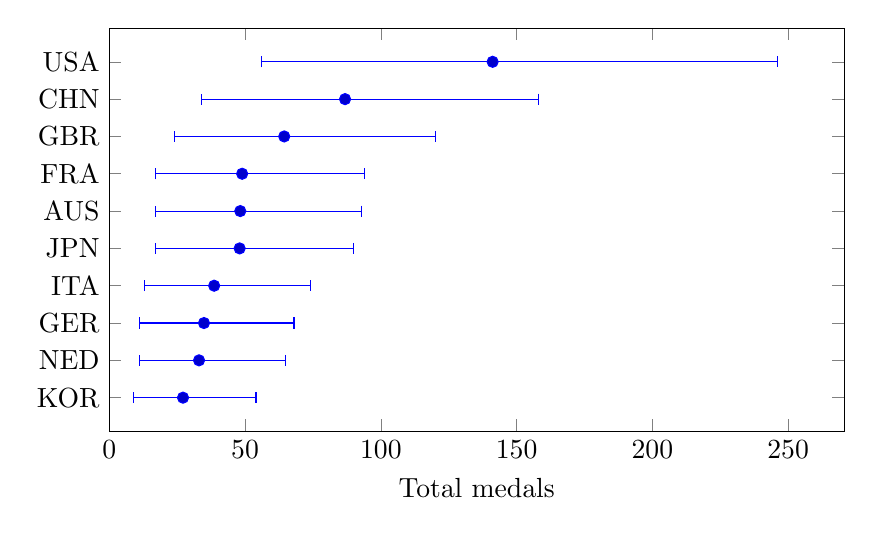
\begin{tikzpicture}\begin{axis}[width=.9\linewidth,height=6.7cm,xlabel={Total medals},symbolic y coords={KOR,NED,GER,ITA,JPN,AUS,FRA,GBR,CHN,USA},ytick=data,xmin=0,error bars/x dir=both,error bars/x explicit]
\addplot+[only marks] coordinates {(27.1348,KOR) += (26.8652,0) -= (18.1348,0) (33.0451,NED) += (31.9549,0) -= (22.0451,0) (34.8625,GER) += (33.1375,0) -= (23.8625,0) (38.6113,ITA) += (35.3887,0) -= (25.6113,0) (47.9943,JPN) += (42.0057,0) -= (30.9943,0) (48.2257,AUS) += (44.7743,0) -= (31.2257,0) (48.9193,FRA) += (45.0807,0) -= (31.9193,0) (64.4164,GBR) += (55.5836,0) -= (40.4164,0) (86.8151,CHN) += (71.1849,0) -= (52.8151,0) (141.1662,USA) += (104.8338,0) -= (85.1662,0)};
\end{axis}\end{tikzpicture}
\caption{Expected total medals and 95\% prediction intervals under the retained-2024 programme and roster scenario.}
\label{fig:2}
\end{figure}
\section{First-medal probabilities}
The candidate set consists of 65 delegates in the retained roster that have never earned a medal under the supplied summer-Games history and explicit code mapping. This is not a claim about winter Games. The conditional participation assumption is essential.

The expected number is 3.3842; the most likely integer is 3, probability 21.71\%. The 95\% predictive interval is [0, 7]. Shared bootstrap fits and fixed-budget allocation mean the count distribution is not formed from independent fixed Bernoulli draws alone.

Leading probabilities are model-based and reflect historical participation features, not scouting of specific athletes. Countries without medals do not receive automatic zero probabilities. Baseline weighted history predicts no first medals, illustrating its limitation.

The saved historical Brier scores and expected versus observed first counts quantify calibration limitations. Roster changes and sparse first-medal observations prevent a precise forecast of the number of successful new delegations.

Figure~\ref{fig:3} provides the corresponding visual comparison.

Table~\ref{tab:4} reports the numerical results.

\begin{table}[htbp]
\centering
\caption{Leading first-medal probabilities in the retained participant roster.}
\label{tab:4}
\small
\begin{tabular}{@{}L{4.122cm} R{6.107cm} R{5.038cm}@{}}
\toprule
NOC & Delegation & First-medal probability\\
\midrule
MLI & Mali & 21.0\%\\
GUI & Guinea & 20.6\%\\
SSD & South Sudan & 16.3\%\\
ANG & Angola & 14.4\%\\
LBR & Liberia & 8.2\%\\
PLE & Palestine & 7.6\%\\
ESA & El Salvador & 7.4\%\\
GAM & Gambia & 7.1\%\\
ARU & Aruba & 6.6\%\\
NEP & Nepal & 6.5\%\\
\bottomrule
\end{tabular}
\end{table}
\begin{figure}[htbp]
\centering
\begin{center}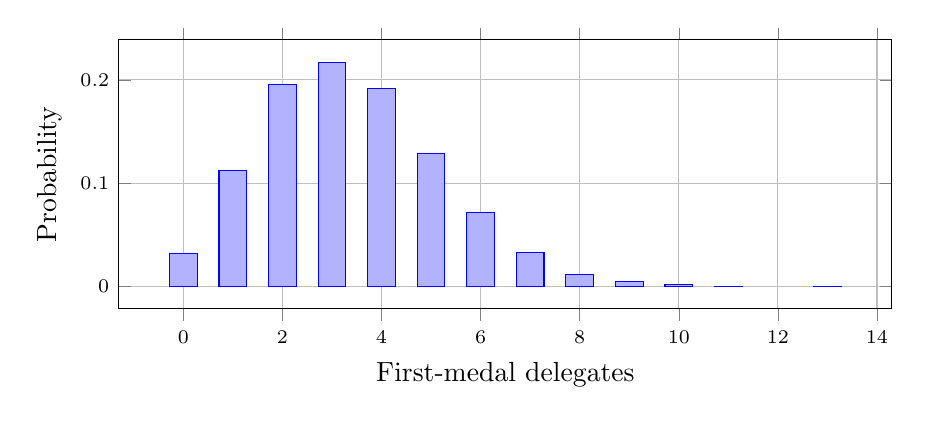
\begin{tikzpicture}\begin{axis}[width=0.94\linewidth,height=5cm,grid=major,legend style={font=\scriptsize},tick label style={font=\scriptsize},ybar,xlabel={First-medal delegates},ylabel={Probability}]
\addplot coordinates {(0,0.032000) (1,0.111900) (2,0.195450) (3,0.217100) (4,0.191250) (5,0.128750) (6,0.071700) (7,0.032900) (8,0.012000) (9,0.005050) (10,0.001600) (11,0.000250) (13,0.000050)};
\end{axis}\end{tikzpicture}\end{center}

\caption{The first-medal count distribution includes shared bootstrap parameters and a fixed joint medal budget.}
\label{fig:3}
\end{figure}
\section{Sport opportunities and host choices}
We aggregate aquatic subdisciplines, gymnastics disciplines, cycling disciplines and other compatible labels into programme sport categories. Recent proxy medal shares use weights 0.6/0.3/0.1 for 2024/2020/2016; participation shares replace medal shares when no medal units exist.

Country exposure changes by the weighted sum of sport event multipliers. Elasticity is assumed equal to one. Expansion scenarios scale the global budget in proportion to the event count; the host-oriented reallocation keeps it fixed. These are stress tests derived from supplied historical categories, not externally sourced 2028 events.

The USA-oriented scenario expands its top three proxy categories (Aquatics, Athletics, Gymnastics) by 10\% while reducing other event opportunities to preserve the overall event total. Gains and losses are redistributed consistently across delegates.

The heatmap identifies which opportunities matter in this constructed model. Because reconstructed sport units do not always equal official national medals, small differences should not be presented as exact sport-level forecasts or causal effects of host selection.

Figure~\ref{fig:4} provides the corresponding visual comparison.

\begin{figure}[htbp]
\centering
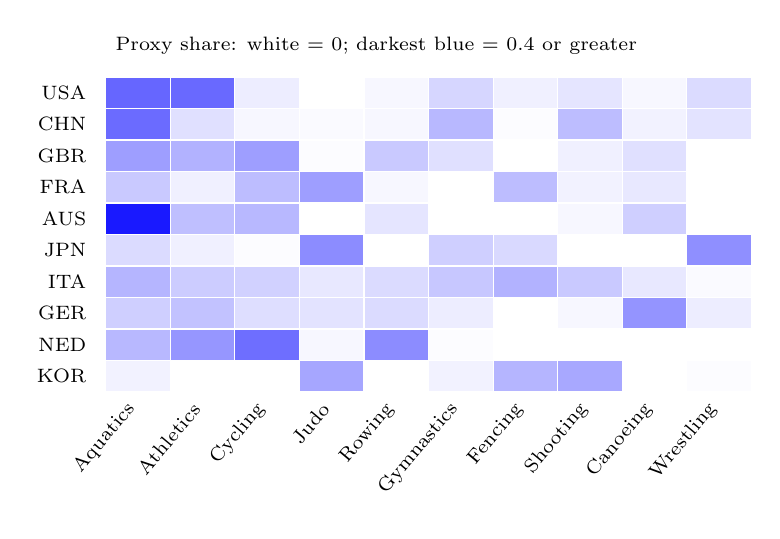
\begin{tikzpicture}[x=0.82cm,y=0.40cm]
\node[rotate=50,anchor=east,font=\scriptsize] at (0.5,-.2) {Aquatics};
\node[rotate=50,anchor=east,font=\scriptsize] at (1.5,-.2) {Athletics};
\node[rotate=50,anchor=east,font=\scriptsize] at (2.5,-.2) {Cycling};
\node[rotate=50,anchor=east,font=\scriptsize] at (3.5,-.2) {Judo};
\node[rotate=50,anchor=east,font=\scriptsize] at (4.5,-.2) {Rowing};
\node[rotate=50,anchor=east,font=\scriptsize] at (5.5,-.2) {Gymnastics};
\node[rotate=50,anchor=east,font=\scriptsize] at (6.5,-.2) {Fencing};
\node[rotate=50,anchor=east,font=\scriptsize] at (7.5,-.2) {Shooting};
\node[rotate=50,anchor=east,font=\scriptsize] at (8.5,-.2) {Canoeing};
\node[rotate=50,anchor=east,font=\scriptsize] at (9.5,-.2) {Wrestling};
\node[anchor=east,font=\scriptsize] at (-.15,9.5) {USA};
\filldraw[fill=blue!60!white,draw=white] (0,9) rectangle (1,10);
\filldraw[fill=blue!59!white,draw=white] (1,9) rectangle (2,10);
\filldraw[fill=blue!7!white,draw=white] (2,9) rectangle (3,10);
\filldraw[fill=blue!0!white,draw=white] (3,9) rectangle (4,10);
\filldraw[fill=blue!3!white,draw=white] (4,9) rectangle (5,10);
\filldraw[fill=blue!16!white,draw=white] (5,9) rectangle (6,10);
\filldraw[fill=blue!6!white,draw=white] (6,9) rectangle (7,10);
\filldraw[fill=blue!10!white,draw=white] (7,9) rectangle (8,10);
\filldraw[fill=blue!3!white,draw=white] (8,9) rectangle (9,10);
\filldraw[fill=blue!14!white,draw=white] (9,9) rectangle (10,10);
\node[anchor=east,font=\scriptsize] at (-.15,8.5) {CHN};
\filldraw[fill=blue!58!white,draw=white] (0,8) rectangle (1,9);
\filldraw[fill=blue!12!white,draw=white] (1,8) rectangle (2,9);
\filldraw[fill=blue!3!white,draw=white] (2,8) rectangle (3,9);
\filldraw[fill=blue!2!white,draw=white] (3,8) rectangle (4,9);
\filldraw[fill=blue!3!white,draw=white] (4,8) rectangle (5,9);
\filldraw[fill=blue!28!white,draw=white] (5,8) rectangle (6,9);
\filldraw[fill=blue!1!white,draw=white] (6,8) rectangle (7,9);
\filldraw[fill=blue!26!white,draw=white] (7,8) rectangle (8,9);
\filldraw[fill=blue!5!white,draw=white] (8,8) rectangle (9,9);
\filldraw[fill=blue!11!white,draw=white] (9,8) rectangle (10,9);
\node[anchor=east,font=\scriptsize] at (-.15,7.5) {GBR};
\filldraw[fill=blue!38!white,draw=white] (0,7) rectangle (1,8);
\filldraw[fill=blue!30!white,draw=white] (1,7) rectangle (2,8);
\filldraw[fill=blue!38!white,draw=white] (2,7) rectangle (3,8);
\filldraw[fill=blue!1!white,draw=white] (3,7) rectangle (4,8);
\filldraw[fill=blue!21!white,draw=white] (4,7) rectangle (5,8);
\filldraw[fill=blue!12!white,draw=white] (5,7) rectangle (6,8);
\filldraw[fill=blue!0!white,draw=white] (6,7) rectangle (7,8);
\filldraw[fill=blue!6!white,draw=white] (7,7) rectangle (8,8);
\filldraw[fill=blue!12!white,draw=white] (8,7) rectangle (9,8);
\filldraw[fill=blue!0!white,draw=white] (9,7) rectangle (10,8);
\node[anchor=east,font=\scriptsize] at (-.15,6.5) {FRA};
\filldraw[fill=blue!21!white,draw=white] (0,6) rectangle (1,7);
\filldraw[fill=blue!6!white,draw=white] (1,6) rectangle (2,7);
\filldraw[fill=blue!26!white,draw=white] (2,6) rectangle (3,7);
\filldraw[fill=blue!38!white,draw=white] (3,6) rectangle (4,7);
\filldraw[fill=blue!3!white,draw=white] (4,6) rectangle (5,7);
\filldraw[fill=blue!0!white,draw=white] (5,6) rectangle (6,7);
\filldraw[fill=blue!26!white,draw=white] (6,6) rectangle (7,7);
\filldraw[fill=blue!5!white,draw=white] (7,6) rectangle (8,7);
\filldraw[fill=blue!9!white,draw=white] (8,6) rectangle (9,7);
\filldraw[fill=blue!0!white,draw=white] (9,6) rectangle (10,7);
\node[anchor=east,font=\scriptsize] at (-.15,5.5) {AUS};
\filldraw[fill=blue!90!white,draw=white] (0,5) rectangle (1,6);
\filldraw[fill=blue!25!white,draw=white] (1,5) rectangle (2,6);
\filldraw[fill=blue!28!white,draw=white] (2,5) rectangle (3,6);
\filldraw[fill=blue!0!white,draw=white] (3,5) rectangle (4,6);
\filldraw[fill=blue!10!white,draw=white] (4,5) rectangle (5,6);
\filldraw[fill=blue!0!white,draw=white] (5,5) rectangle (6,6);
\filldraw[fill=blue!0!white,draw=white] (6,5) rectangle (7,6);
\filldraw[fill=blue!3!white,draw=white] (7,5) rectangle (8,6);
\filldraw[fill=blue!19!white,draw=white] (8,5) rectangle (9,6);
\filldraw[fill=blue!0!white,draw=white] (9,5) rectangle (10,6);
\node[anchor=east,font=\scriptsize] at (-.15,4.5) {JPN};
\filldraw[fill=blue!14!white,draw=white] (0,4) rectangle (1,5);
\filldraw[fill=blue!6!white,draw=white] (1,4) rectangle (2,5);
\filldraw[fill=blue!1!white,draw=white] (2,4) rectangle (3,5);
\filldraw[fill=blue!45!white,draw=white] (3,4) rectangle (4,5);
\filldraw[fill=blue!0!white,draw=white] (4,4) rectangle (5,5);
\filldraw[fill=blue!19!white,draw=white] (5,4) rectangle (6,5);
\filldraw[fill=blue!15!white,draw=white] (6,4) rectangle (7,5);
\filldraw[fill=blue!0!white,draw=white] (7,4) rectangle (8,5);
\filldraw[fill=blue!0!white,draw=white] (8,4) rectangle (9,5);
\filldraw[fill=blue!44!white,draw=white] (9,4) rectangle (10,5);
\node[anchor=east,font=\scriptsize] at (-.15,3.5) {ITA};
\filldraw[fill=blue!29!white,draw=white] (0,3) rectangle (1,4);
\filldraw[fill=blue!20!white,draw=white] (1,3) rectangle (2,4);
\filldraw[fill=blue!18!white,draw=white] (2,3) rectangle (3,4);
\filldraw[fill=blue!9!white,draw=white] (3,3) rectangle (4,4);
\filldraw[fill=blue!14!white,draw=white] (4,3) rectangle (5,4);
\filldraw[fill=blue!22!white,draw=white] (5,3) rectangle (6,4);
\filldraw[fill=blue!30!white,draw=white] (6,3) rectangle (7,4);
\filldraw[fill=blue!21!white,draw=white] (7,3) rectangle (8,4);
\filldraw[fill=blue!9!white,draw=white] (8,3) rectangle (9,4);
\filldraw[fill=blue!2!white,draw=white] (9,3) rectangle (10,4);
\node[anchor=east,font=\scriptsize] at (-.15,2.5) {GER};
\filldraw[fill=blue!19!white,draw=white] (0,2) rectangle (1,3);
\filldraw[fill=blue!24!white,draw=white] (1,2) rectangle (2,3);
\filldraw[fill=blue!13!white,draw=white] (2,2) rectangle (3,3);
\filldraw[fill=blue!11!white,draw=white] (3,2) rectangle (4,3);
\filldraw[fill=blue!14!white,draw=white] (4,2) rectangle (5,3);
\filldraw[fill=blue!7!white,draw=white] (5,2) rectangle (6,3);
\filldraw[fill=blue!0!white,draw=white] (6,2) rectangle (7,3);
\filldraw[fill=blue!3!white,draw=white] (7,2) rectangle (8,3);
\filldraw[fill=blue!42!white,draw=white] (8,2) rectangle (9,3);
\filldraw[fill=blue!7!white,draw=white] (9,2) rectangle (10,3);
\node[anchor=east,font=\scriptsize] at (-.15,1.5) {NED};
\filldraw[fill=blue!28!white,draw=white] (0,1) rectangle (1,2);
\filldraw[fill=blue!41!white,draw=white] (1,1) rectangle (2,2);
\filldraw[fill=blue!57!white,draw=white] (2,1) rectangle (3,2);
\filldraw[fill=blue!3!white,draw=white] (3,1) rectangle (4,2);
\filldraw[fill=blue!45!white,draw=white] (4,1) rectangle (5,2);
\filldraw[fill=blue!1!white,draw=white] (5,1) rectangle (6,2);
\filldraw[fill=blue!0!white,draw=white] (6,1) rectangle (7,2);
\filldraw[fill=blue!0!white,draw=white] (7,1) rectangle (8,2);
\filldraw[fill=blue!0!white,draw=white] (8,1) rectangle (9,2);
\filldraw[fill=blue!0!white,draw=white] (9,1) rectangle (10,2);
\node[anchor=east,font=\scriptsize] at (-.15,0.5) {KOR};
\filldraw[fill=blue!5!white,draw=white] (0,0) rectangle (1,1);
\filldraw[fill=blue!0!white,draw=white] (1,0) rectangle (2,1);
\filldraw[fill=blue!0!white,draw=white] (2,0) rectangle (3,1);
\filldraw[fill=blue!35!white,draw=white] (3,0) rectangle (4,1);
\filldraw[fill=blue!0!white,draw=white] (4,0) rectangle (5,1);
\filldraw[fill=blue!5!white,draw=white] (5,0) rectangle (6,1);
\filldraw[fill=blue!29!white,draw=white] (6,0) rectangle (7,1);
\filldraw[fill=blue!34!white,draw=white] (7,0) rectangle (8,1);
\filldraw[fill=blue!0!white,draw=white] (8,0) rectangle (9,1);
\filldraw[fill=blue!1!white,draw=white] (9,0) rectangle (10,1);
\node[anchor=west,font=\scriptsize] at (0,11) {Proxy share: white = 0; darkest blue = 0.4 or greater};
\end{tikzpicture}
\caption{Recent sport proxy shares describe programme exposure; they are not exact official sport-level medal allocations.}
\label{fig:4}
\end{figure}
\section{Coaching evidence and investment scenarios}
No coach name or appointment date is provided. We search for changes in two-edition sport proxy rates, adjust opportunities and compare country-wide official strength. This produces candidate positive excesses. Appointment, athlete quality, federation investment and rule changes remain unobserved confounders.

For example, the leading candidate CHN / Gymnastics has a positive proxy excess 12.65 across two post-change editions. Assigning 0-100\% of that excess to coaching is only an attribution scenario, not an identified causal bound. We cannot estimate a defensible pure great-coach contribution from these data alone.

We select three delegates with an active 2024 programme and a historically established sport with a recent proxy shortfall. This avoids proposing coaching-only gains for a sport with no current participation. Recommended cases are Japan: Aquatics; Jamaica: Athletics; Poland: Athletics.

Assuming 10\%, 20\% or 30\% sport-strength uplift, we scale the country sport share and redistribute the fixed total budget. The table shows the 20\% case. These expected gains are conditional arithmetic, not measured coach effects, salaries, return on investment or guaranteed medals.

Figure~\ref{fig:5} provides the corresponding visual comparison.

Table~\ref{tab:5} reports the numerical results.

\begin{table}[htbp]
\centering
\caption{Coaching investment scenarios assuming a 20\% sport-strength uplift.}
\label{tab:5}
\small
\begin{tabular}{@{}L{5.119cm} R{3.312cm} R{3.312cm} R{3.312cm}@{}}
\toprule
Delegation & Sport & Base total & 20\% case gain\\
\midrule
Japan & Aquatics & 47.99 & 0.57\\
Jamaica & Athletics & 7.43 & 1.47\\
Poland & Athletics & 11.24 & 0.71\\
\bottomrule
\end{tabular}
\par\smallskip{\footnotesize Note. Gains are assumed scenarios, not identified coaching effects.}
\end{table}
\begin{figure}[htbp]
\centering
\begin{center}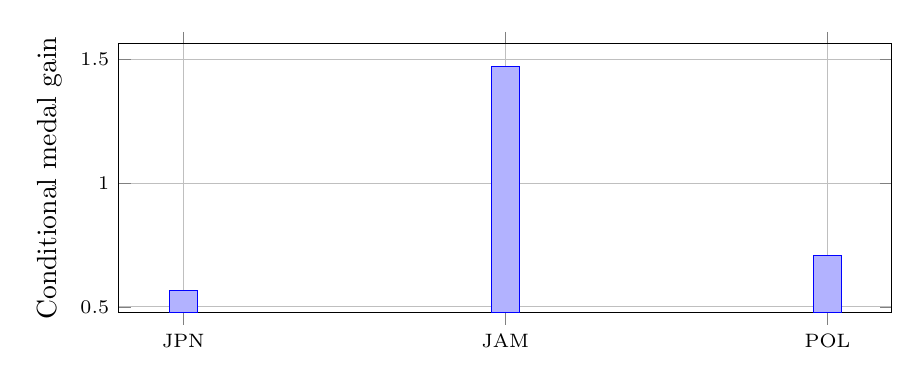
\begin{tikzpicture}\begin{axis}[width=0.94\linewidth,height=5cm,grid=major,legend style={font=\scriptsize},tick label style={font=\scriptsize},ybar,symbolic x coords={JPN,JAM,POL},xtick=data,ylabel={Conditional medal gain}]
\addplot coordinates {(JPN,0.56599) (JAM,1.47240) (POL,0.70795)};
\end{axis}\end{tikzpicture}\end{center}

\caption{Conditional gains follow an assumed 20\% sport-strength uplift; these are not estimated coach causal effects.}
\label{fig:5}
\end{figure}
\section{An exploratory insight: specialization and volatility}
Among 65 delegates with four recent observations and average total at least two, the correlation between recent sport specialization HHI and medal-count coefficient of variation is Spearman rho=0.483, nominal p=4.69e-05.

HHI is the sum of squared recent sport proxy shares; volatility uses official totals for 2012-2024. The positive relationship suggests that concentrated programmes may be more exposed to the performance of a small set of sports. It is a descriptive association, not proof that diversification causes stability.

The windows overlap, the sample is selected, proxies have measurement error and multiple insights were considered. Wealth, programme size and organizational differences are not observed. The nominal p-value does not resolve these limitations.

An Olympic committee can use this as a prompt for stress testing: quantify the loss if one dominant sport underperforms, then compare a targeted specialization strategy with a portfolio of realistic second-strength sports.

Figure~\ref{fig:6} provides the corresponding visual comparison.

\begin{figure}[htbp]
\centering
\begin{center}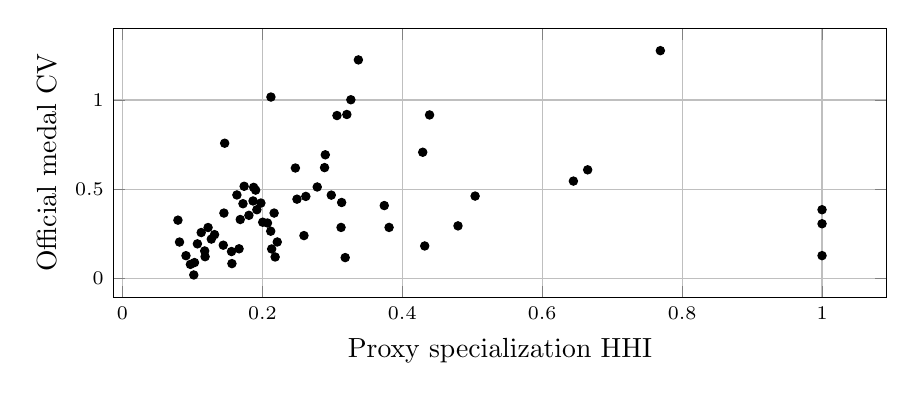
\begin{tikzpicture}\begin{axis}[width=0.94\linewidth,height=5cm,grid=major,legend style={font=\scriptsize},tick label style={font=\scriptsize},xlabel={Proxy specialization HHI},ylabel={Official medal CV}]
\addplot[only marks,mark size=1.5pt] coordinates {(0.21332,0.16496) (0.31250,0.28571) (0.21198,0.26459) (0.21228,1.01663) (0.27846,0.51239) (0.24950,0.44412) (0.10303,0.08872) (0.42925,0.70711) (0.18670,0.43401) (0.16675,0.16593) (0.11818,0.12173) (0.21684,0.36623) (0.12708,0.22036) (0.25950,0.24000) (0.20736,0.31052) (0.11265,0.25713) (0.28893,0.62103) (0.33728,1.22474) (0.18080,0.35355) (0.09717,0.07857) (1.00000,0.38490) (0.07937,0.32646) (0.10202,0.01928) (0.31845,0.11664) (0.09085,0.12735) (0.17401,0.51640) (0.32653,1.00138) (0.21831,0.12001) (0.38117,0.28571) (0.19793,0.42235) (0.47966,0.29439) (0.29855,0.46681) (0.32079,0.91879) (0.08162,0.20377) (1.00000,0.30626) (0.10720,0.19369) (0.17234,0.41860) (1.00000,0.12766) (0.76889,1.27657) (0.13169,0.24527) (0.19043,0.49487) (0.64461,0.54545) (0.20054,0.31492) (0.66500,0.60858) (0.16844,0.33011) (0.19217,0.38490) (0.14417,0.18614) (0.43901,0.91625) (0.15592,0.15061) (0.28999,0.69282) (0.37429,0.40825) (0.26215,0.45957) (0.22133,0.20412) (0.14509,0.36623) (0.16365,0.46771) (0.50413,0.46154) (0.11760,0.15385) (0.31337,0.42552) (0.14617,0.75768) (0.43210,0.18182) (0.18759,0.51031) (0.12245,0.28520) (0.15652,0.08299) (0.24724,0.61881) (0.30667,0.91287)};
\end{axis}\end{tikzpicture}\end{center}

\caption{Sport concentration and official medal volatility are positively associated in the selected 65-delegation sample.}
\label{fig:6}
\end{figure}
\section{Sensitivity, ablation and interval checks}
We refit on training starts 1996, 2000 and 2004, remove the USA host indicator, and inspect sport-opportunity alternatives. Sensitivity point means normalize gold and non-gold budgets separately; they are not identical to bootstrap predictive means.

The current-host multiplier is exp(bH)=1.173. Edition-bootstrap 95\% percentiles are [1.055, 1.312]. This is a conditional model association based on few hosts, not a causal hosting estimate.

Removing host, participant or sport-breadth terms is evaluated on the same four validation editions. The anchored established-delegate mean primarily uses history and host; participant and sport ablations affect the rare-delegate count submodel. Small differences are therefore expected.

We also check budget allocation using preceding-edition budgets in each retrospective forecast. Because future event budgets and participation remain unknown, process-only historical coverage does not certify the wider conditional 2028 intervals.

Figure~\ref{fig:7} provides the corresponding visual comparison.

Table~\ref{tab:6} reports the numerical results.

\begin{table}[htbp]
\centering
\caption{Ablation errors averaged over the four validation editions.}
\label{tab:6}
\small
\begin{tabular}{@{}L{4.122cm} R{6.107cm} R{5.038cm}@{}}
\toprule
Removed & Total MAE & Gold MAE\\
\midrule
athletes & 1.661 & 0.740\\
host & 1.670 & 0.756\\
sports & 1.661 & 0.740\\
\bottomrule
\end{tabular}
\end{table}
\begin{figure}[htbp]
\centering
\begin{center}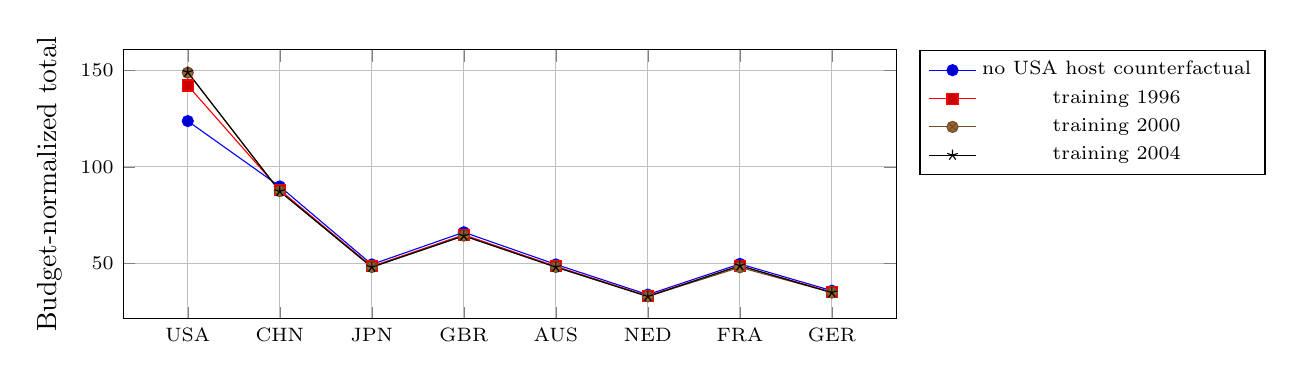
\begin{tikzpicture}\begin{axis}[width=0.94\linewidth,height=5cm,grid=major,legend style={font=\scriptsize},tick label style={font=\scriptsize},symbolic x coords={USA,CHN,JPN,GBR,AUS,NED,FRA,GER},xtick=data,ylabel={Budget-normalized total},legend pos=outer north east]
\addplot coordinates {(USA,123.7407) (CHN,89.8390) (JPN,49.3668) (GBR,66.0791) (AUS,49.3823) (NED,33.7136) (FRA,49.6379) (GER,35.7532)};\addlegendentry{no USA host counterfactual}
\addplot coordinates {(USA,142.1897) (CHN,88.0139) (JPN,48.3633) (GBR,64.7509) (AUS,48.3849) (NED,33.0307) (FRA,48.6411) (GER,35.0313)};\addlegendentry{training 1996}
\addplot coordinates {(USA,148.8484) (CHN,87.3738) (JPN,48.0113) (GBR,64.2863) (AUS,48.0356) (NED,32.7913) (FRA,47.8741) (GER,34.7785)};\addlegendentry{training 2000}
\addplot coordinates {(USA,149.0993) (CHN,87.2394) (JPN,47.9375) (GBR,64.1855) (AUS,47.9609) (NED,32.7406) (FRA,48.7413) (GER,34.7244)};\addlegendentry{training 2004}
\end{axis}\end{tikzpicture}\end{center}

\caption{Budget-normalized point forecasts vary with training windows and the USA host indicator.}
\label{fig:7}
\end{figure}
\section{Limitations and committee recommendations}
The simplest weighted-history model has better point MAE than the selected task-complete model. We report this clearly. Choosing a richer model serves first-medal probability, host response and a joint distribution; it does not make point forecasts universally more accurate.

The 2028 roster, participant scale and programme are assumed, and the primary budget is fixed. Athletes and events may change substantially. Confidence about country rankings is limited by broad intervals, sparse editions, proxy inconsistency and unobserved institutional changes.

The latest historical check was inspected in development. A truly prospective evaluation would require new data not yet used for model design. Raw-data anomalies and country-code changes can also affect first-medal classification.

Committees should use the strong simple benchmark for a reference, the joint model for uncertainty and scenario planning, and the sport matrix for exposure analysis. Prioritize evidence-backed programmes rather than buying a coach based on a residual alone. Monitor participant depth and medal concentration, then revise scenarios when legitimate future information becomes available.

For the exercise, quantitative inputs remain limited to the supplied files. External GDP, live athlete rankings and actual future sport lists are not added to the model. All figures and table numbers are generated from saved computations \cite{comap-problem,comap-data,nb2-doc}.

\section{Reproducibility and references}
Run scripts/run\_all.py with the project .venv Python to rebuild audits, features, rolling comparisons, forecasts, bootstrap draws, scenarios and figures. Run unittest discovery in tests for raw input integrity, future-label perturbation, probability bounds and joint budget constraints. Run scripts/build\_report.py to regenerate this report.

Random seed is 20251009; final simulation uses seed offsets recorded in source. requirements-lock.txt pins actual installed packages. logs/last\_run.json records execution duration and environment. source\_manifest.json and official\_data\_comparison.json link the supplied bytes to official ZIP contents.

Table~\ref{tab:7} reports the numerical results.

\begin{table}[htbp]
\centering
\caption{Joint-budget retrospective forecasts retaining the preceding edition budget.}
\label{tab:7}
\small
\begin{tabular}{@{}L{5.119cm} R{3.312cm} R{3.312cm} R{3.312cm}@{}}
\toprule
Edition & Total MAE & Gold MAE & Total 95\% coverage\\
\midrule
2008 & 1.560 & 0.672 & 97.5\%\\
2012 & 1.353 & 0.668 & 97.5\%\\
2016 & 1.381 & 0.613 & 97.5\%\\
2020 & 1.714 & 0.787 & 95.2\%\\
2024 & 1.520 & 0.686 & 96.1\%\\
\bottomrule
\end{tabular}
\end{table}
\begin{thebibliography}{9}
\bibitem{comap-problem}COMAP. 2025 MCM Problem C: Models for Olympic Medal Tables. Local official problem PDF, especially pages 2-3. Official archive: \url{https://www.contest.comap.org/undergraduate/contests/mcm/contests/2025/problems/}
\bibitem{comap-data}COMAP. 2025 Problem C Data.zip: summerOly\_athletes, summerOly\_medal\_counts, summerOly\_hosts, summerOly\_programs and data\_dictionary. Local files are byte-identical to the official archive. No other quantitative dataset is used.
\bibitem{nb2-doc}Statsmodels documentation: NegativeBinomial (NB2 variance) and Binomial families. \url{https://www.statsmodels.org/stable/generated/statsmodels.discrete.discrete_model.NegativeBinomial.html} . Numerical optimization uses SciPy; specific objective functions and regularization are implemented in source.
\bibitem{codex-use}OpenAI Codex, AI-assisted model implementation, analysis and writing, 9 October 2026. Exact runtime model identifiers are not exposed to these scripts; the user requested GPT-6.1 Sol during the session. See the appended AI-use record.
\bibitem{comap-ai}COMAP. Use of AI Tools in COMAP Contests, v102025, retrieved 9 October 2026. \url{https://www.contest.comap.com/undergraduate/contests/mcm/flyer/Contest_AI_Policy.pdf} . The retrieved policy is not claimed to be the original January 2025 policy version.
\end{thebibliography}
\clearpage
\appendix
\section{Complete delegation forecasts}
\subsection*{1-41}
Expected medals and 95\% joint prediction intervals. All results are conditional on retained 2024 roster, programme and reported-delegation budgets. Full precision, improvement probabilities and scenarios are in CSV.

Table~\ref{tab:8} reports the numerical results.

{\small\begin{longtable}{@{}L{1.098cm} L{4.464cm} R{1.463cm} R{2.195cm} R{1.610cm} R{2.342cm}@{}}
\caption{Complete delegation forecasts: 1-41.}\label{tab:8}\\
\toprule
NOC & Delegation & Gold & Gold 95\% & Total & Total 95\%\\
\midrule
\endhead
USA & United States & 46.61 & [17, 83] & 141.17 & [56, 246]\\
CHN & China & 37.16 & [14, 68] & 86.82 & [34, 158]\\
JPN & Japan & 20.99 & [7, 41] & 47.99 & [17, 90]\\
GBR & Great Britain & 17.49 & [5, 34] & 64.42 & [24, 120]\\
AUS & Australia & 16.51 & [5, 33] & 48.23 & [17, 93]\\
NED & Netherlands & 12.71 & [3, 26] & 33.05 & [11, 65]\\
FRA & France & 12.64 & [3, 26] & 48.92 & [17, 94]\\
GER & Germany & 11.76 & [3, 25] & 34.86 & [11, 68]\\
ITA & Italy & 10.92 & [3, 23] & 38.61 & [13, 74]\\
KOR & South Korea & 10.42 & [3, 22] & 27.13 & [9, 54]\\
NZL & New Zealand & 8.40 & [2, 18] & 19.61 & [6, 40]\\
CAN & Canada & 7.81 & [2, 17] & 25.46 & [8, 51]\\
HUN & Hungary & 6.14 & [1, 14] & 18.74 & [6, 38]\\
UZB & Uzbekistan & 6.06 & [1, 14] & 10.59 & [3, 23]\\
ESP & Spain & 4.55 & [1, 11] & 17.48 & [5, 36]\\
BRA & Brazil & 4.53 & [1, 11] & 20.11 & [6, 41]\\
KEN & Kenya & 4.18 & [0, 10] & 10.93 & [3, 23]\\
CUB & Cuba & 3.73 & [0, 9] & 10.94 & [3, 23]\\
NOR & Norway & 3.61 & [0, 9] & 7.62 & [2, 17]\\
SWE & Sweden & 3.49 & [0, 9] & 10.42 & [3, 22]\\
CZE & Czech Republic & 3.10 & [0, 8] & 7.33 & [2, 16]\\
IRL & Ireland & 3.02 & [0, 8] & 5.67 & [1, 13]\\
IRI & Iran & 2.98 & [0, 8] & 10.02 & [2, 21]\\
SRB & Serbia & 2.90 & [0, 8] & 6.52 & [1, 15]\\
BEL & Belgium & 2.87 & [0, 8] & 8.65 & [2, 19]\\
BUL & Bulgaria & 2.69 & [0, 7] & 6.30 & [1, 14]\\
CRO & Croatia & 2.60 & [0, 7] & 7.60 & [2, 17]\\
GEO & Georgia & 2.60 & [0, 7] & 7.30 & [2, 16]\\
JAM & Jamaica & 2.41 & [0, 7] & 7.43 & [2, 17]\\
UKR & Ukraine & 2.31 & [0, 6] & 13.94 & [4, 29]\\
DEN & Denmark & 2.30 & [0, 6] & 10.21 & [2, 22]\\
ROU & Romania & 2.24 & [0, 6] & 7.08 & [1, 16]\\
SLO & Slovenia & 2.22 & [0, 6] & 3.78 & [0, 9]\\
POL & Poland & 2.02 & [0, 6] & 11.24 & [3, 24]\\
TPE & Chinese Taipei & 1.92 & [0, 5] & 8.14 & [2, 18]\\
SUI & Switzerland & 1.81 & [0, 5] & 9.41 & [2, 20]\\
INA & Indonesia & 1.65 & [0, 5] & 3.72 & [0, 9]\\
HKG & Hong Kong & 1.55 & [0, 5] & 4.32 & [0, 10]\\
PHI & Philippines & 1.55 & [0, 5] & 3.84 & [0, 9]\\
GRE & Greece & 1.54 & [0, 5] & 6.65 & [1, 15]\\
AUT & Austria & 1.52 & [0, 5] & 5.21 & [1, 12]\\
\bottomrule
\end{longtable}}
\par\smallskip{\footnotesize Note. Point estimates are simulation means; intervals are conditional predictive quantiles.}
\clearpage
\subsection*{42-82}
Expected medals and 95\% joint prediction intervals. All results are conditional on retained 2024 roster, programme and reported-delegation budgets. Full precision, improvement probabilities and scenarios are in CSV.

Table~\ref{tab:9} reports the numerical results.

{\small\begin{longtable}{@{}L{1.098cm} L{4.464cm} R{1.463cm} R{2.195cm} R{1.610cm} R{2.342cm}@{}}
\caption{Complete delegation forecasts: 42-82.}\label{tab:9}\\
\toprule
NOC & Delegation & Gold & Gold 95\% & Total & Total 95\%\\
\midrule
\endhead
BRN & Bahrain & 1.35 & [0, 4] & 3.03 & [0, 8]\\
AZE & Azerbaijan & 1.34 & [0, 4] & 8.08 & [2, 18]\\
UGA & Uganda & 1.26 & [0, 4] & 2.53 & [0, 7]\\
ECU & Ecuador & 1.26 & [0, 4] & 4.03 & [0, 10]\\
ALG & Algeria & 1.25 & [0, 4] & 2.14 & [0, 6]\\
ISR & Israel & 1.24 & [0, 4] & 5.69 & [1, 13]\\
THA & Thailand & 1.15 & [0, 4] & 4.86 & [1, 11]\\
RSA & South Africa & 1.14 & [0, 4] & 5.58 & [1, 13]\\
ETH & Ethiopia & 1.04 & [0, 3] & 4.49 & [0, 11]\\
MAR & Morocco & 0.97 & [0, 3] & 1.74 & [0, 5]\\
TUN & Tunisia & 0.96 & [0, 3] & 2.83 & [0, 7]\\
ARG & Argentina & 0.95 & [0, 3] & 3.23 & [0, 8]\\
EGY & Egypt & 0.95 & [0, 3] & 3.99 & [0, 10]\\
POR & Portugal & 0.94 & [0, 3] & 3.79 & [0, 9]\\
KAZ & Kazakhstan & 0.84 & [0, 3] & 8.36 & [2, 18]\\
BAH & Bahamas & 0.76 & [0, 3] & 0.88 & [0, 3]\\
KOS & Kosovo & 0.75 & [0, 3] & 2.05 & [0, 6]\\
TUR & Turkey & 0.74 & [0, 3] & 9.58 & [2, 21]\\
PAK & Pakistan & 0.69 & [0, 3] & 0.69 & [0, 3]\\
DMA & Dominica & 0.68 & [0, 3] & 0.68 & [0, 3]\\
GUA & Guatemala & 0.66 & [0, 3] & 1.32 & [0, 4]\\
CHI & Chile & 0.66 & [0, 3] & 1.34 & [0, 4]\\
BOT & Botswana & 0.66 & [0, 3] & 1.64 & [0, 5]\\
QAT & Qatar & 0.65 & [0, 3] & 1.74 & [0, 5]\\
LCA & Saint Lucia & 0.65 & [0, 3] & 1.32 & [0, 4]\\
DOM & Dominican Republic & 0.64 & [0, 3] & 3.50 & [0, 9]\\
SVK & Slovakia & 0.54 & [0, 2] & 2.35 & [0, 6]\\
FIJ & Fiji & 0.44 & [0, 2] & 1.43 & [0, 4]\\
PUR & Puerto Rico & 0.44 & [0, 2] & 1.72 & [0, 5]\\
BER & Bermuda & 0.38 & [0, 2] & 0.38 & [0, 2]\\
EST & Estonia & 0.35 & [0, 2] & 0.81 & [0, 3]\\
LAT & Latvia & 0.35 & [0, 2] & 0.70 & [0, 3]\\
VEN & Venezuela & 0.33 & [0, 2] & 1.62 & [0, 5]\\
COL & Colombia & 0.33 & [0, 2] & 4.73 & [1, 11]\\
IND & India & 0.33 & [0, 2] & 5.93 & [1, 14]\\
PRK & North Korea & 0.22 & [0, 1] & 4.37 & [0, 10]\\
VIE & Vietnam & 0.14 & [0, 1] & 0.28 & [0, 2]\\
JOR & Jordan & 0.12 & [0, 1] & 1.42 & [0, 4]\\
SGP & Singapore & 0.12 & [0, 1] & 0.81 & [0, 3]\\
TJK & Tajikistan & 0.11 & [0, 1] & 2.00 & [0, 6]\\
CIV & Cote d'Ivoire & 0.11 & [0, 1] & 1.20 & [0, 4]\\
\bottomrule
\end{longtable}}
\par\smallskip{\footnotesize Note. Point estimates are simulation means; intervals are conditional predictive quantiles.}
\clearpage
\subsection*{83-123}
Expected medals and 95\% joint prediction intervals. All results are conditional on retained 2024 roster, programme and reported-delegation budgets. Full precision, improvement probabilities and scenarios are in CSV.

Table~\ref{tab:10} reports the numerical results.

{\small\begin{longtable}{@{}L{1.098cm} L{4.464cm} R{1.463cm} R{2.195cm} R{1.610cm} R{2.342cm}@{}}
\caption{Complete delegation forecasts: 83-123.}\label{tab:10}\\
\toprule
NOC & Delegation & Gold & Gold 95\% & Total & Total 95\%\\
\midrule
\endhead
ARM & Armenia & 0.11 & [0, 1] & 4.05 & [0, 10]\\
MLI & Mali & 0.09 & [0, 1] & 0.28 & [0, 2]\\
GUI & Guinea & 0.09 & [0, 1] & 0.28 & [0, 2]\\
SSD & South Sudan & 0.07 & [0, 1] & 0.20 & [0, 2]\\
ANG & Angola & 0.07 & [0, 1] & 0.19 & [0, 2]\\
LBR & Liberia & 0.03 & [0, 1] & 0.10 & [0, 1]\\
PLE & Palestine & 0.03 & [0, 1] & 0.09 & [0, 1]\\
ESA & El Salvador & 0.03 & [0, 1] & 0.08 & [0, 1]\\
GAM & Gambia & 0.03 & [0, 1] & 0.08 & [0, 1]\\
GUM & Guam & 0.03 & [0, 0] & 0.07 & [0, 1]\\
GBS & Guinea Bissau & 0.03 & [0, 0] & 0.07 & [0, 1]\\
ARU & Aruba & 0.02 & [0, 0] & 0.08 & [0, 1]\\
VAN & Vanuatu & 0.02 & [0, 0] & 0.07 & [0, 1]\\
NEP & Nepal & 0.02 & [0, 0] & 0.07 & [0, 1]\\
MAD & Madagascar & 0.02 & [0, 0] & 0.07 & [0, 1]\\
RWA & Rwanda & 0.02 & [0, 0] & 0.07 & [0, 1]\\
PNG & Papua New Guinea & 0.02 & [0, 0] & 0.07 & [0, 1]\\
LBA & Libya & 0.02 & [0, 0] & 0.07 & [0, 1]\\
MON & Monaco & 0.02 & [0, 0] & 0.06 & [0, 1]\\
NCA & Nicaragua & 0.02 & [0, 0] & 0.06 & [0, 1]\\
MHL & Marshall Islands & 0.02 & [0, 0] & 0.06 & [0, 1]\\
MOZ & Mozambique & 0.02 & [0, 0] & 0.06 & [0, 1]\\
TOG & Togo & 0.02 & [0, 0] & 0.06 & [0, 1]\\
ERI & Eritrea & 0.02 & [0, 0] & 0.06 & [0, 1]\\
LIB & Lebanon & 0.02 & [0, 0] & 0.06 & [0, 1]\\
MLT & Malta & 0.02 & [0, 0] & 0.05 & [0, 1]\\
CRC & Costa Rica & 0.02 & [0, 0] & 0.06 & [0, 1]\\
LUX & Luxembourg & 0.02 & [0, 0] & 0.05 & [0, 1]\\
CAF & Central African Republic & 0.02 & [0, 0] & 0.06 & [0, 1]\\
ISL & Iceland & 0.02 & [0, 0] & 0.05 & [0, 1]\\
ZIM & Zimbabwe & 0.02 & [0, 0] & 0.05 & [0, 1]\\
COD & Congo (Kinshasa) & 0.02 & [0, 0] & 0.06 & [0, 1]\\
CMR & Cameroon & 0.02 & [0, 0] & 0.05 & [0, 1]\\
TGA & Tonga & 0.02 & [0, 0] & 0.06 & [0, 1]\\
AFG & Afghanistan & 0.02 & [0, 0] & 0.05 & [0, 1]\\
TAN & Tanzania & 0.02 & [0, 0] & 0.05 & [0, 1]\\
MDV & Maldives & 0.02 & [0, 0] & 0.06 & [0, 1]\\
IRQ & Iraq & 0.02 & [0, 0] & 0.05 & [0, 1]\\
SUR & Suriname & 0.02 & [0, 0] & 0.06 & [0, 1]\\
SAM & Samoa & 0.02 & [0, 0] & 0.06 & [0, 1]\\
SRI & Sri Lanka & 0.02 & [0, 0] & 0.05 & [0, 1]\\
\bottomrule
\end{longtable}}
\par\smallskip{\footnotesize Note. Point estimates are simulation means; intervals are conditional predictive quantiles.}
\clearpage
\subsection*{124-164}
Expected medals and 95\% joint prediction intervals. All results are conditional on retained 2024 roster, programme and reported-delegation budgets. Full precision, improvement probabilities and scenarios are in CSV.

Table~\ref{tab:11} reports the numerical results.

{\small\begin{longtable}{@{}L{1.098cm} L{4.464cm} R{1.463cm} R{2.195cm} R{1.610cm} R{2.342cm}@{}}
\caption{Complete delegation forecasts: 124-164.}\label{tab:11}\\
\toprule
NOC & Delegation & Gold & Gold 95\% & Total & Total 95\%\\
\midrule
\endhead
MNE & Montenegro & 0.02 & [0, 0] & 0.05 & [0, 1]\\
HAI & Haiti & 0.02 & [0, 0] & 0.05 & [0, 1]\\
URU & Uruguay & 0.02 & [0, 0] & 0.05 & [0, 1]\\
CGO & Congo (Brazzaville) & 0.02 & [0, 0] & 0.05 & [0, 1]\\
TLS & Timor Leste & 0.02 & [0, 0] & 0.05 & [0, 1]\\
SUD & Sudan & 0.02 & [0, 0] & 0.05 & [0, 1]\\
COM & Comoros & 0.02 & [0, 0] & 0.05 & [0, 1]\\
GAB & Gabon & 0.02 & [0, 0] & 0.06 & [0, 1]\\
VIN & Saint Vincent and the Grenadines & 0.02 & [0, 0] & 0.05 & [0, 1]\\
GUY & Guyana & 0.02 & [0, 0] & 0.05 & [0, 1]\\
ISV & United States Virgin Islands & 0.02 & [0, 0] & 0.05 & [0, 1]\\
SEN & Senegal & 0.02 & [0, 0] & 0.05 & [0, 1]\\
PAR & Paraguay & 0.02 & [0, 0] & 0.05 & [0, 1]\\
BAR & Barbados & 0.02 & [0, 0] & 0.05 & [0, 1]\\
BIH & Bosnia and Herzegovina & 0.02 & [0, 0] & 0.05 & [0, 1]\\
ANT & Antigua and Barbuda & 0.02 & [0, 0] & 0.05 & [0, 1]\\
SLE & Sierra Leone & 0.02 & [0, 0] & 0.04 & [0, 1]\\
DJI & Djibouti & 0.02 & [0, 0] & 0.05 & [0, 1]\\
BAN & Bangladesh & 0.02 & [0, 0] & 0.05 & [0, 1]\\
MRI & Mauritius & 0.02 & [0, 0] & 0.05 & [0, 1]\\
BOL & Bolivia & 0.02 & [0, 0] & 0.04 & [0, 1]\\
IVB & British Virgin Islands & 0.02 & [0, 0] & 0.05 & [0, 1]\\
LAO & Laos & 0.02 & [0, 0] & 0.04 & [0, 1]\\
BRU & Brunei & 0.02 & [0, 0] & 0.04 & [0, 1]\\
OMA & Oman & 0.02 & [0, 0] & 0.04 & [0, 1]\\
SKN & Saint Kitts and Nevis & 0.02 & [0, 0] & 0.05 & [0, 1]\\
BEN & Benin & 0.02 & [0, 0] & 0.05 & [0, 1]\\
YEM & Yemen & 0.01 & [0, 0] & 0.04 & [0, 1]\\
CAY & Cayman Islands & 0.01 & [0, 0] & 0.04 & [0, 1]\\
CHA & Chad & 0.01 & [0, 0] & 0.04 & [0, 1]\\
FSM & Federated States of Micronesia & 0.01 & [0, 0] & 0.04 & [0, 1]\\
LES & Lesotho & 0.01 & [0, 0] & 0.04 & [0, 1]\\
CAM & Cambodia & 0.01 & [0, 0] & 0.04 & [0, 1]\\
PLW & Palau & 0.01 & [0, 0] & 0.04 & [0, 1]\\
GEQ & Equatorial Guinea & 0.01 & [0, 0] & 0.04 & [0, 1]\\
KIR & Kiribati & 0.01 & [0, 0] & 0.04 & [0, 1]\\
STP & Sao Tome and Principe & 0.01 & [0, 0] & 0.04 & [0, 1]\\
BHU & Bhutan & 0.01 & [0, 0] & 0.04 & [0, 1]\\
SWZ & Swaziland & 0.01 & [0, 0] & 0.04 & [0, 1]\\
MTN & Mauritania & 0.01 & [0, 0] & 0.03 & [0, 1]\\
TUV & Tuvalu & 0.01 & [0, 0] & 0.03 & [0, 1]\\
\bottomrule
\end{longtable}}
\par\smallskip{\footnotesize Note. Point estimates are simulation means; intervals are conditional predictive quantiles.}
\clearpage
\subsection*{165-205}
Expected medals and 95\% joint prediction intervals. All results are conditional on retained 2024 roster, programme and reported-delegation budgets. Full precision, improvement probabilities and scenarios are in CSV.

Table~\ref{tab:12} reports the numerical results.

{\small\begin{longtable}{@{}L{1.098cm} L{4.464cm} R{1.463cm} R{2.195cm} R{1.610cm} R{2.342cm}@{}}
\caption{Complete delegation forecasts: 165-205.}\label{tab:12}\\
\toprule
NOC & Delegation & Gold & Gold 95\% & Total & Total 95\%\\
\midrule
\endhead
SEY & Seychelles & 0.01 & [0, 0] & 0.03 & [0, 1]\\
MYA & Myanmar & 0.01 & [0, 0] & 0.03 & [0, 1]\\
AND & Andorra & 0.01 & [0, 0] & 0.03 & [0, 1]\\
MAW & Malawi & 0.01 & [0, 0] & 0.03 & [0, 1]\\
SOL & Solomon Islands & 0.01 & [0, 0] & 0.03 & [0, 1]\\
HON & Honduras & 0.01 & [0, 0] & 0.03 & [0, 0]\\
COK & Cook Islands & 0.01 & [0, 0] & 0.02 & [0, 0]\\
SOM & Somalia & 0.01 & [0, 0] & 0.02 & [0, 0]\\
ASA & American Samoa & 0.01 & [0, 0] & 0.02 & [0, 0]\\
NRU & Nauru & 0.01 & [0, 0] & 0.02 & [0, 0]\\
BIZ & Belize & 0.01 & [0, 0] & 0.02 & [0, 0]\\
LIE & Liechtenstein & 0.01 & [0, 0] & 0.02 & [0, 0]\\
MEX & Mexico & 0.00 & [0, 0] & 4.73 & [1, 11]\\
KGZ & Kyrgyzstan & 0.00 & [0, 0] & 4.54 & [1, 11]\\
MAS & Malaysia & 0.00 & [0, 0] & 2.39 & [0, 6]\\
MDA & Moldova & 0.00 & [0, 0] & 2.79 & [0, 7]\\
LTU & Lithuania & 0.00 & [0, 0] & 3.16 & [0, 8]\\
MGL & Mongolia & 0.00 & [0, 0] & 2.08 & [0, 6]\\
GRN & Grenada & 0.00 & [0, 0] & 1.71 & [0, 5]\\
ALB & Albania & 0.00 & [0, 0] & 1.29 & [0, 4]\\
CPV & Cape Verde & 0.00 & [0, 0] & 0.70 & [0, 3]\\
SMR & San Marino & 0.00 & [0, 0] & 1.00 & [0, 3]\\
FIN & Finland & 0.00 & [0, 0] & 0.80 & [0, 3]\\
EOR & EOR & 0.00 & [0, 0] & 0.70 & [0, 3]\\
PAN & Panama & 0.00 & [0, 0] & 0.69 & [0, 3]\\
NGR & Nigeria & 0.00 & [0, 0] & 0.79 & [0, 3]\\
PER & Peru & 0.00 & [0, 0] & 0.70 & [0, 3]\\
BUR & Burkina Faso & 0.00 & [0, 0] & 0.38 & [0, 2]\\
CYP & Cyprus & 0.00 & [0, 0] & 0.69 & [0, 3]\\
ZAM & Zambia & 0.00 & [0, 0] & 0.69 & [0, 3]\\
KSA & Saudi Arabia & 0.00 & [0, 0] & 0.38 & [0, 2]\\
KUW & Kuwait & 0.00 & [0, 0] & 0.38 & [0, 2]\\
MKD & Macedonia & 0.00 & [0, 0] & 0.38 & [0, 2]\\
NAM & Namibia & 0.00 & [0, 0] & 0.39 & [0, 2]\\
SYR & Syria & 0.00 & [0, 0] & 0.38 & [0, 2]\\
TKM & Turkmenistan & 0.00 & [0, 0] & 0.38 & [0, 2]\\
NIG & Niger & 0.00 & [0, 0] & 0.16 & [0, 1]\\
GHA & Ghana & 0.00 & [0, 0] & 0.38 & [0, 2]\\
BDI & Burundi & 0.00 & [0, 0] & 0.16 & [0, 1]\\
TTO & Trinidad and Tobago & 0.00 & [0, 0] & 0.16 & [0, 1]\\
UAE & United Arab Emirates & 0.00 & [0, 0] & 0.16 & [0, 1]\\
\bottomrule
\end{longtable}}
\par\smallskip{\footnotesize Note. Point estimates are simulation means; intervals are conditional predictive quantiles.}
\clearpage
\section*{Report on Use of AI Tools}
\addcontentsline{toc}{section}{Report on Use of AI Tools}
Tool: OpenAI Codex. Date: 9 October 2026. The user requested GPT-6.1 Sol after the initial implementation; the exact active runtime model is not exposed to the numerical process and should be confirmed from the application for any formal citation.

Known user requests (English translations): start modeling; switch to GPT-6.1 Sol; continue modeling. Exact Chinese wording is preserved in the companion AI-use record. Earlier prompts requested local 2025 problem analysis and a standalone C-problem execution plan. AI was used for planning, Python implementation, data handling, model design, interpretation, figure generation, Chinese explanation and English writing \cite{codex-use}.

Substantive generated outputs are preserved in src/, scripts/, tests/, report/, the execution plan and this PDF. Computation inputs are only the five supplied CSV files; retrieved documentation supports implementation and disclosure, not extra numerical predictors.

Verification performed: source hashes, numerical rerun, historical comparisons, probability and joint-budget checks, and visual report review. These do not replace human review of assumptions. No student identities, control number, submission or human approval have been invented.

This is a transparent training reconstruction, not a certified contest submission. The short record does not reproduce the entire conversation. For formal use, export and retain the full conversation, exact model/version details and complete generated outputs, and adapt the disclosure to the applicable policy \cite{comap-ai}.

\end{document}